\documentclass[a4paper,10pt]{article}
\usepackage[utf8]{inputenc}
 
% Blank line between paragraphs instead of indenting the first line
\usepackage{parskip}
\setlength{\parskip}{\baselineskip}

% Squash a bit more text onto a page
\usepackage{geometry}
\geometry{verbose,tmargin=20mm,bmargin=20mm,lmargin=25mm,rmargin=25mm}

\usepackage{graphicx}
\usepackage{listings}
\usepackage{amsmath}
\usepackage{verbatim}

% Indent verbatim environments
\makeatletter \def\verbatim@processline{\hspace*{2em}\the\verbatim@line\par}\makeatother

\lstdefinelanguage{logicdef}
{
  morekeywords={DEVICES, MONITORS, CONNECTIONS, END},
  sensitive=false,
  morecomment=[s]{/*}{*/},
  basicstyle=\small\ttfamily,
  keywordstyle=\pmb,
  frame=single,
  numbers=left,
  numberstyle=\tiny
}



\begin{document}

\begin{center}
\LARGE \textbf{IIA GF2 Software: 1st interim report}

\small Team 8 - Martin Jackson (mj380), Tim Hillel (th389) and Jamie Magee (jam96)
\end{center}



\section{Introduction}

This project aims to develop a logic simulation program, involving all five major phases of the software engineering life cycle: specification, design, implementation, testing and maintenance.

This report focuses on the specification phase, providing the EBNF for syntax, an informal description of semantics and a description of the error handling, as well as example definition files.
Details of teamwork planning are also provided.

\section{General approach}

The project was broken into individual tasks within each phase of the software life cyle.
The timeframe was then decided for each task and each task was assigned to either a team member or the whole team, depending on the nature of the task.
This is shown in Figure~\ref{fig:ganttchart} of Appendix~\ref{appendix:gantt}.

Each member of the team was also assigned a general project role as follows:

\textbf{Project manager:} (T Hillel) - Responsible for project planning including delegation of tasks and ensuring that the project runs to the set timescale.

\textbf{Programming administrator:} (J Magee) - Responsible for upkeep of the project directory including performing builds and keeping legacy versions of the simulator.

\textbf{Client representative:} (M Jackson) - Responsible for ensuring that the project meets the client's requirements for the logic simulator as defined in Appendix A of the GF2 Project Handout.

\section{Syntax and semantics}

\begin{verbatim}
specfile = devices connections monitors
devices = 'DEVICES' dev {';' dev} 'END'
connections = 'CONNECTIONS' [con] {';' con} 'END' 
monitors = 'MONITORS' [mon] {';' mon} 'END'
\end{verbatim} 

\textbf{Semantics:} None.
%An input file is composed of one devices, one connections and one monitors block, in that order. The devices block must contain at least one \texttt{dev}, but the connections and monitors blocks may be empty. Each block is started with `\texttt{DEVICES}', `\texttt{CONNECTIONS}' and `\texttt{MONITORS}' respectively, and each block is terminated with `\texttt{END}'.

\begin{verbatim}
dev = clock|switch|gate|dtype|xor
clock = 'CLOCK' devicename':'digit{digit}
switch = 'SWITCH' devicename':'('0'|'1')
gate = ('AND'|'NAND'|'OR'|'NOR') devicename':'('1'|'2'|'3'|'4'|'5'|'6'|
       '7'|'8'|'9'|'10'|'11'|'12'|'13'|'14'|'15'|'16')
dtype = 'DTYPE' devicename
xor = 'XOR' devicename
\end{verbatim} 

\textbf{Semantics:} These statements define a new device of the specified type. Each \texttt{devicename} must be unique, and must not be \texttt{DEVICES}, \texttt{CONNECTIONS}, \texttt{MONITORS}, \texttt{END}, \texttt{CLOCK}, \texttt{SWITCH}, \texttt{AND}, \texttt{NAND}, \texttt{OR}, \texttt{NOR}, \texttt{DTYPE} or \texttt{XOR}, as these are reserved words.
Each \texttt{devicename} referred to in the connections or monitors block must first be defined in the devices block. \texttt{devicename} is case sensitive. For a \texttt{CLOCK}, the integer parameter must be greater than zero, and represents the number of simulation cycles between output state changes. For \texttt{SWITCH} devices, the parameter is the initial state of the device (1 is on, 0 is off).
For logic gates (\texttt{AND}, \texttt{NAND}, \texttt{OR}, \texttt{NOR}), the parameter is the number of inputs.

\begin{verbatim}
con = devicename'.'input '=' devicename['.'output]
\end{verbatim} 
\textbf{Semantics:} Connects the specified device input to the specified device output. Multiple inputs may be connected to the same output, but attempting to connect multiple outputs to the same input is a semantic error. Multiple definitions of the same connection (i.e. the same input and output as an existing connection) will generate a warning, and are treated as a single instance of the connection. For an explanation of warnings and errors, see section~\ref{sec:error-handling}. All inputs must be connected. See below for semantic rules for \verb|devicename'.'input| and \verb|devicename['.'output]|.

\begin{verbatim}
mon = devicename['.'output]
\end{verbatim} 
\textbf{Semantics:} Adds an output signal to the list of signals to be monitored. Multiple monitor statements for the same output signal generate a warning, but are allowed.

\begin{verbatim}
devicename = letter {'_'|letter|digit}
\end{verbatim}
\textbf{Semantics:} Semantics for \texttt{devicename} are described above, in the description of \texttt{dev} statements.

\begin{verbatim}
input = 'I'('1'|'2'|'3'|'4'|'5'|'6'|'7'|'8'|'9'|'10'|'11'|'12'|'13'|'14'|
        '15'|'16')|'DATA'|'CLK'|'SET'|'CLEAR'
output = 'Q'['BAR']
\end{verbatim} 

\textbf{Semantics:} \verb|devicename'.'input| indicates an input pin on a device. The input pin must be valid according to the properties of the device that \texttt{devicename} refers to. For example, for a gate defined to have 4 inputs, only \texttt{I1}, \texttt{I2}, \texttt{I3}, and \texttt{I4} may be used; and \texttt{DATA}, \texttt{CLK}, \texttt{SET}, and \texttt{CLEAR} may only be used when \texttt{devicename} is a \texttt{DTYPE}.
Note that this rule prevents input to a \texttt{CLOCK} or \texttt{SWITCH}, as there are no valid input pin names for those devices.

\verb|devicename['.'output]| indicates an output pin on a device. \texttt{output} must be given when \texttt{devicename} is a \texttt{DTYPE} (the only device with more than one output), otherwise \texttt{output} must be omitted. 

Comments start with \texttt{/*} and are terminated by the first \texttt{*/}. A \texttt{/*} inside a comment is ignored. 

\section{Error handling}
\label{sec:error-handling}

For all errors, the definition file will continue to be read as far as possible and further errors will be reported. However, running the simulation is not allowed until the errors have been fixed and the file loaded again. Duplicate connections or monitors result in a warning. Warnings still allow the simulation to be run. 

If a semicolon is omitted, an error message should be printed and text should be skipped until the next semicolon is found. Scanning should then continue as normal. A missing semicolon will be detected by the occurrence of a syntax error. After reading as many symbols as are allowed by the syntax rules in a \texttt{dev}, \texttt{con} or \texttt{mon} statement, the next symbol expected is either \texttt{END} or a semicolon. If the next symbol is neither of these, then a semicolon has been omitted. 

If a \texttt{dev}, \texttt{con}, or \texttt{mon} statement does not conform to the correct syntax, then it will be ignored, an error message will be printed, and scanning will continue after the next semicolon. 

If statements are present outside a devices, connections, or monitors block, then an error message will be printed and they will be ignored. Scanning will continue at the next \texttt{DEVICES}, \texttt{CONNECTIONS}, or \texttt{MONITORS} keyword. 

If \texttt{DEVICES}, \texttt{CONNECTIONS}, or \texttt{MONITORS} keyword appears without using \texttt{END} to terminate the previous block, an error message will be printed and scanning will continue as though the previous block was correctly terminated. 

If a comment is not terminated before the end of the file, then an error message will be printed. The contents of the comment will still be ignored.

If an end comment symbol (\texttt{*/}) is detected without a preceding start comment symbol (\texttt{/*}), an error message will be generated. Scanning will then continue as normal after the end comment symbol. 
%MAYBE IGNORE TEXT BEFORE \texttt{*/} DISCUSS? There's no particularly good way to determine where to start ignoring it though. The program will probably ignore far too much of the definition file.
%Also, the scanner will already have passed the preceding symbols to the parser, so they can't be ignored. 

For all errors, the error message will include the line number and indicate the position on that line of the error, as well as a description of which error has occurred. 

\clearpage
\appendix

\section{Appendix: Gantt chart}
\label{appendix:gantt}
\begin{figure}[h]
 \centering
  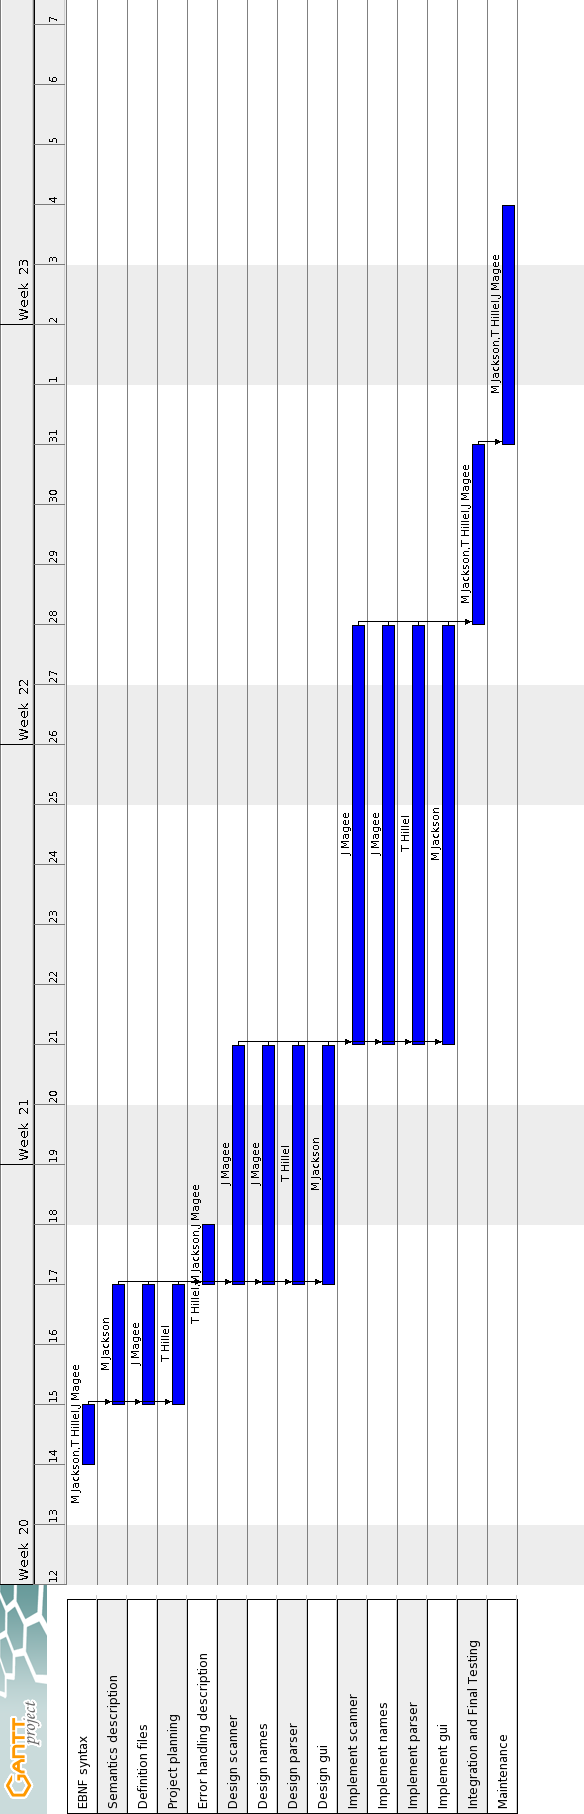
\includegraphics[height=19cm]{Gantt-Chart.png}
 \caption{Gantt chart showing key events in development cycle}
 \label{fig:ganttchart}
\end{figure}

\clearpage

\section{Appendix: examples}

\subsection{Example circuit diagrams}
\begin{figure}[h]
 \centering
 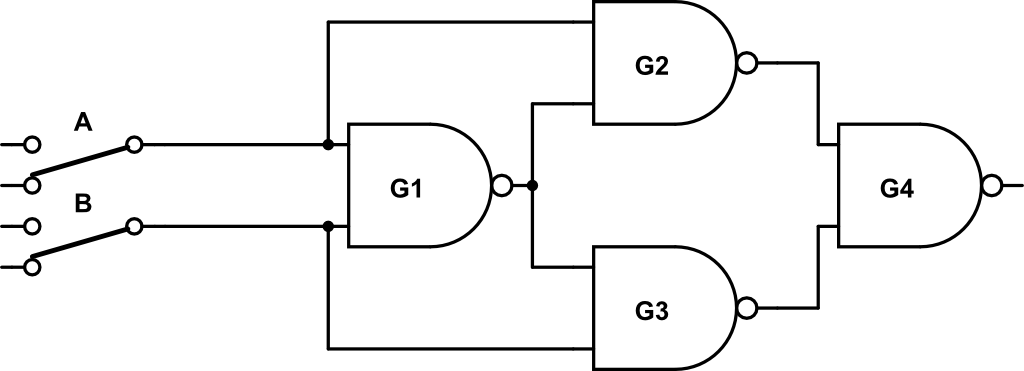
\includegraphics[width=14cm]{../examples/xor.png}
 \caption{Circuit diagram of an XOR gate implemented using NAND gates}
 \label{fig:example-xor}
\end{figure}

\begin{figure}[h]
 \centering
 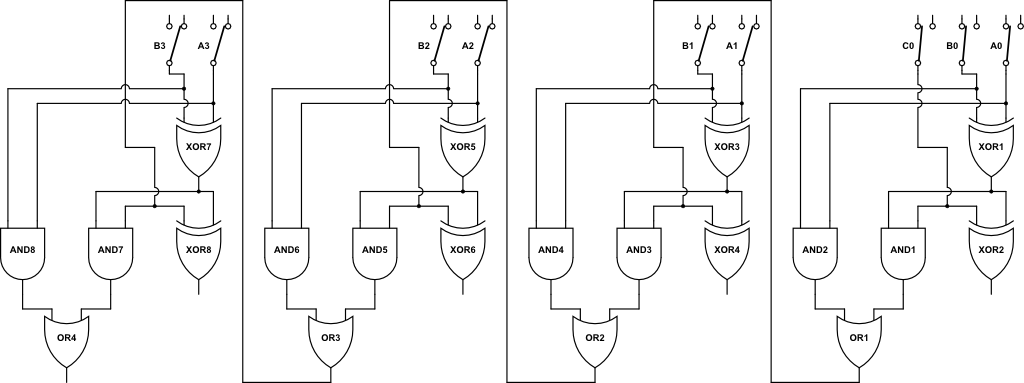
\includegraphics[width=16cm]{../examples/4-bit-adder.png}
 \caption{Circuit diagram of a 4 bit adder}
 \label{fig:example-adder}
\end{figure}


\subsection{Example definition file for XOR gate circuit}
\lstinputlisting[language=logicdef]{../examples/xor.txt}

\subsection{Example definition file for 4 bit adder circuit}
\lstinputlisting[language=logicdef]{../examples/4bitadder.txt}

\section{Appendix: EBNF}
\verbatiminput{../docs/ebnf.txt}

\end{document}


